%% This is an example first chapter.  You should put chapter/appendix that you
%% write into a separate file, and add a line \include{yourfilename} to
%% main.tex, where `yourfilename.tex' is the name of the chapter/appendix file.
%% You can process specific files by typing their names in at the 
%% \files=
%% prompt when you run the file main.tex through LaTeX.

\chapter{Introduction}

The cost effectiveness and reachability of COTS elements, shrinking size of electronics serve as a perfect environment for small flying vehicles to emerge. 
This accelerating trend towards small but capable flying vehicles is pushing the limits of both hardware and software potentials of industry and academia. 
Increasing usage of these vehicles for a variety of missions pushes a further liability to secure the flight. With the advent of the new era of UAS, different institutions all over the world, specifically National Aeronautics and Space Administration (NASA) 
\cite{kopardekarunmanned} and Federal Aviation Administration (FAA) \cite{FAA_UASintegration} in US, European Aviation Safety Agency (EASA) \cite{A_NPA_EASA2015} in Europe and international bases such as International Civil Aviation Organization (ICAO) \cite{ICAO_Circular} are addressing safe integration of UAS in airspace \cite{baskaya2016flexible}.

\section{Motivation}

Improvement of the reliability of the flight is considered to be one of the main goals for integrating UAVs into civil airspace according to Unmanned systems roadmap by US Office of the Secretary of Defense, DoD \cite{UnmannedSystemsRoadmapDoD}. 
To achieve a safe flight is not an easy task considering the unknowns of the systems hardware, environment and possible system faults and failures to emerge. 
Also, increasing demand on cost effective systems, resulting in the smaller sensors and actuators with less accuracy, impose the software to achieve even more. 
The expectation that UAVs should be less expensive than their manned counterparts might have a hit on reliability of the system. Cost saving measures other than the need to support a pilot/crew onboard or decrement in size would probably lead to decrease in system reliability.

Under the research and development programs and initiatives identified by DoD in order to develop technologies and capabilities for UAS, the biggest chunk in control technologies is the health management and adaptive control with a budget of 74.3 M dollars. 
Other safety features such as validation and verification of flight critical intelligent software is the second with 57.8 M dollars \cite{UnmannedSystemsRoadmapDoD}. 

With the last turn in popularity and practicality contest among research topics of the last decade, machine learning and drones seem to be neck to neck. The sides of the race are mostly supported by high tech rather than the public who has concerns in both opponents. Is there a chance that these two can run side by side with cheers? Machine learning guides various aspects of our lives even without noticing it due to its abrupt introduction via the bigger tech companies. Its abilities rise, defeating 9-dan Go professional, their accuracy increase, enabling smooth voice recognition, adding intelligence to our daily lives. Another machine, who wants to enjoy this enabling technology is a drone. Drones, although still very strictly regulated in most countries have been spreading with great passion along their enthusiasts. Machine learning has already started to take part in aviation.

Systems are often susceptible to faults of different nature. Existing irregularities in 
sensors, actuators, or controller Fig.~\ref{fig:faultsInTheSystem} could be amplified due to the control system design 
and lead to failures. A fault could be hidden thanks to the control action \cite{ducard2009fault}.

\begin{figure}
\begin{center}
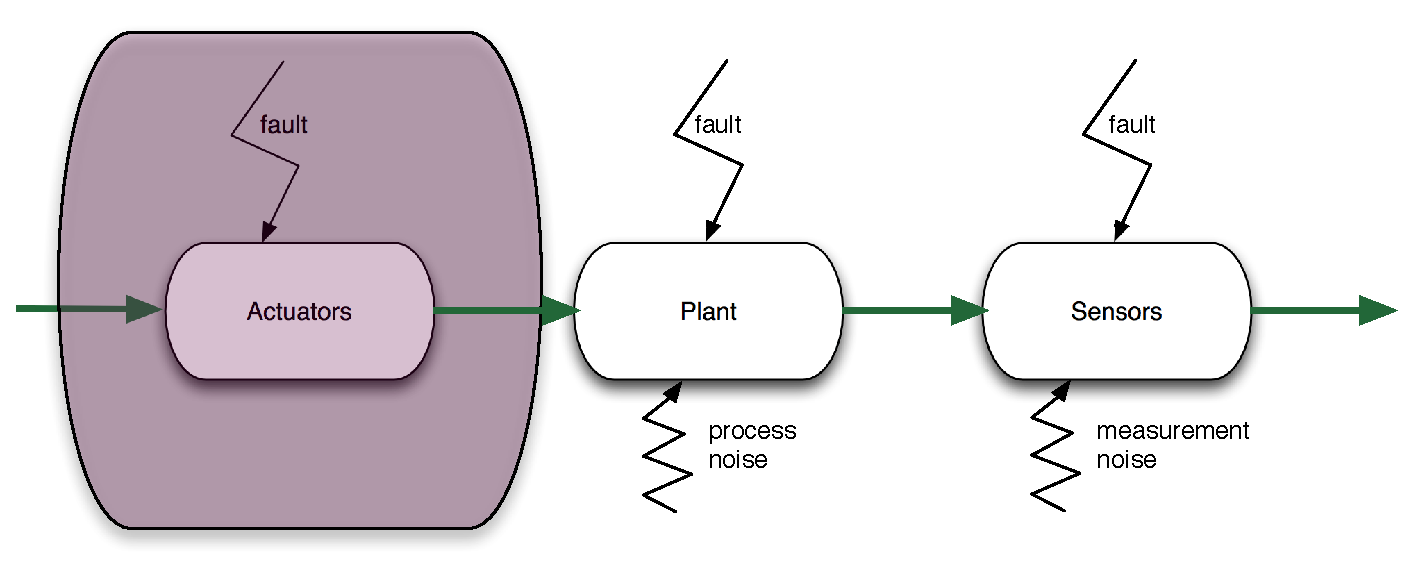
\includegraphics[width=15cm]{figures/faultsInTheSystem}    % The printed column width is 8.4 cm.
\caption{Faults altering the system } 
\label{fig:faultsInTheSystem}
\end{center}
\end{figure}


